\chapter{Перпендикуляр к плоскости и наклонные к ней}\label{ch:ch2}

\begingroup
% Интервалы вокруг рисунков в главе с десятью схемами.
\setlength{\intextsep}{10pt plus 2pt minus 2pt}
\setlength{\textfloatsep}{12pt plus 2pt minus 2pt}

% А. П. Киселёв, «Элементарная геометрия», 23-е издание, 1914. Печатные с. 275–282.
% Номера страниц DjVu на Wikimedia Commons на 11 больше печатных.
\newcommand*{\kiselevPlanimetryPage}[2]{%
    \href{https://commons.wikimedia.org/wiki/File:\%D0\%90._\%D0\%9F._\%D0\%9A\%D0\%B8\%D1\%81\%D0\%B5\%D0\%BB\%D1\%91\%D0\%B2._\%D0\%AD\%D0\%BB\%D0\%B5\%D0\%BC\%D0\%B5\%D0\%BD\%D1\%82\%D0\%B0\%D1\%80\%D0\%BD\%D0\%B0\%D1\%8F_\%D0\%B3\%D0\%B5\%D0\%BE\%D0\%BC\%D0\%B5\%D1\%82\%D1\%80\%D0\%B8\%D1\%8F_(1914).djvu?page=#1}{#2}%
}

% Печатная с. 275.
\kiselevparagraph{para:constructing-plane-normal} \textbf{Предварительное замечание.} Возьмём прямую \(AB\) (рис.~\ref{fig:kiselev-stereo-304}) и проведём через неё две произвольные плоскости \(P\) и \(Q\). Выберем на \(AB\) точку \(C\) и проведём через неё в плоскостях \(P\) и \(Q\) прямые \(CD\perp AB\) и \(CE\perp AB\) соответственно. Через пересекающиеся прямые \(CD\) и \(CE\) проведём плоскость \(R\) (\hyperref[item:plane-through-intersecting-lines]{см.~§~\ref*{para:plane-uniqueness-corollaries}, пункт~\ref*{item:plane-through-intersecting-lines}}). В результате прямая \(AB\) пересекает плоскость \(R\) и перпендикулярна двум прямым \(CD\) и \(CE\), проведённым в этой плоскости через точку пересечения. Докажем, что такое расположение прямой и плоскости обладает следующим важным свойством.

\begin{figure}[htbp]
    \centering
    \renewcommand{\thefigure}{304}
    \captionsetup{name=Рис.,labelsep=period}
    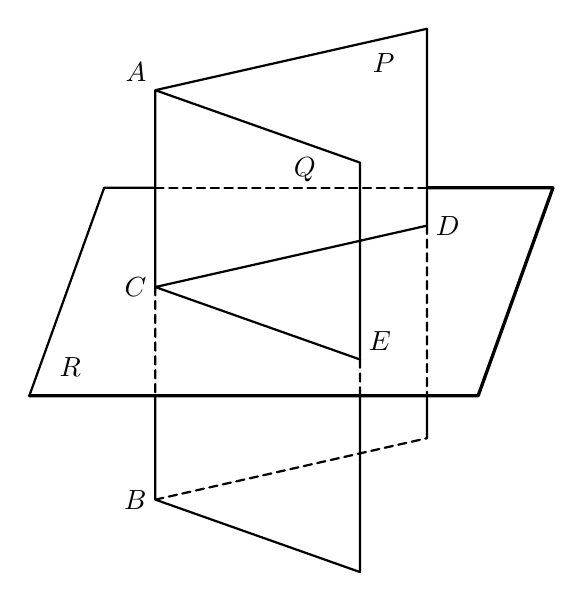
\begin{tikzpicture}[line cap=round,line join=round,every node/.style={inner sep=3pt}]
    \coordinate (A) at (-1.4,2.5);
    \coordinate (B) at (-1.4,-2.7);
    \coordinate (C) at (-1.4,0);
    \coordinate (D) at (2.05,0.78);
    \coordinate (E) at (1.2,-0.92);
    \coordinate (Pbottom) at (2.05,-1.92);
    \coordinate (Qbottom) at (1.2,-3.62);

    % Плоскость R и скрытая часть её заднего края.
    \draw[thick] (-1.4,1.26) -- (-2.05,1.26) -- (-3,-1.38);
    \draw[thick,densely dashed] (-1.4,1.26) -- (2.05,1.26);
    \draw[very thick] (-3,-1.38) -- (2.7,-1.38) -- (3.65,1.26) -- (2.05,1.26);

    % Плоскости P и Q проходят через общую прямую AB.
    \draw[thick] (A) -- (2.05,3.28) -- (D) -- (C)
        (A) -- (1.2,1.58) -- (E) -- (C) -- (A);
    \draw[thick,densely dashed] (C) -- (-1.4,-1.38)
        (D) -- (2.05,-1.38) (E) -- (1.2,-1.38) (B) -- (Pbottom);
    \draw[thick] (-1.4,-1.38) -- (B) -- (Qbottom) -- (1.2,-1.38)
        (2.05,-1.38) -- (Pbottom);

    \node[above left] at (A) {\(A\)};
    \node[left] at (B) {\(B\)};
    \node[left] at (C) {\(C\)};
    \node[right] at (D) {\(D\)};
    \node[above right] at (E) {\(E\)};
    \node at (1.5,2.85) {\(P\)};
    \node at (0.5,1.49) {\(Q\)};
    \node at (-2.48,-1.02) {\(R\)};
\end{tikzpicture}

    \caption{Расположение прямой \(AB\) и плоскости \(R\)}\label{fig:kiselev-stereo-304}
\end{figure}

\kiselevparagraph{para:perpendicular-plane-criterion} \textbf{Теорема. Если прямая} (\(AA_1\), рис.~\ref{fig:kiselev-stereo-305})\textbf{, пересекающая плоскость} \(P\)\textbf{, перпендикулярна двум прямым} (\(CD\) и \(EF\))\textbf{, проведённым в этой плоскости через точку пересечения} \(B\)\textbf{, то она перпендикулярна и любой третьей прямой} \(MN\)\textbf{, проведённой в плоскости через ту же точку пересечения.}

\begin{figure}[htbp]
    \centering
    \renewcommand{\thefigure}{305}
    \captionsetup{name=Рис.,labelsep=period}
    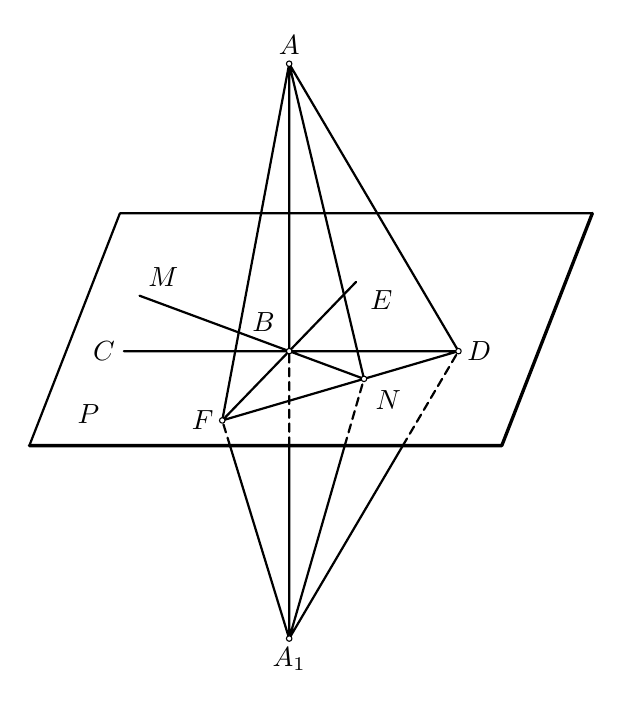
\begin{tikzpicture}[line cap=round,line join=round,every node/.style={inner sep=3pt}]
    \coordinate (A) at (0,3.65);
    \coordinate (A1) at (0,-3.65);
    \coordinate (B) at (0,0);
    \coordinate (C) at (-2.1,0);
    \coordinate (D) at (2.15,0);
    \coordinate (E) at (0.85,0.88);
    \coordinate (F) at (-0.85,-0.88);
    \coordinate (M) at (-1.9,0.704);
    \path (D) -- (F) coordinate[pos=0.4] (N);

    \draw[thick] (-3.3,-1.2) -- (-2.15,1.75) -- (3.85,1.75);
    \draw[very thick] (-3.3,-1.2) -- (2.7,-1.2) -- (3.85,1.75);
    \draw[thick] (C) -- (D) (E) -- (F) (M) -- (N) (D) -- (F);

    \draw[thick] (B) -- (A) -- (D) (A) -- (N) (A) -- (F);
    % Разрывы линий к A_1 показывают, где они скрыты плоскостью P.
    \path (A1) -- (D) coordinate[pos=0.6712] (frontD);
    \path (A1) -- (N) coordinate[pos=0.7429] (frontN);
    \path (A1) -- (F) coordinate[pos=0.8845] (frontF);
    \coordinate (frontB) at (0,-1.2);
    \draw[thick] (A1) -- (frontB) (A1) -- (frontD) (A1) -- (frontN) (A1) -- (frontF);
    \draw[thick,densely dashed] (frontB) -- (B) (frontD) -- (D)
        (frontN) -- (N) (frontF) -- (F);

    \foreach \point in {A,A1,B,D,F,N} {
        \filldraw[fill=white] (\point) circle[radius=1pt];
    }
    \node[above] at (A) {\(A\)};
    \node[below] at (A1) {\(A_1\)};
    \node[above left,xshift=-2pt,yshift=4pt] at (B) {\(B\)};
    \node[left] at (C) {\(C\)};
    \node[right] at (D) {\(D\)};
    \node[below right,xshift=2pt] at (E) {\(E\)};
    \node[left] at (F) {\(F\)};
    \node[above right] at (M) {\(M\)};
    \node[below right,xshift=1pt,yshift=-1pt] at (N) {\(N\)};
    \node at (-2.55,-0.8) {\(P\)};
\end{tikzpicture}

    \caption{Прямая \(AA_1\), перпендикулярная к \(CD\) и \(EF\)}\label{fig:kiselev-stereo-305}
\end{figure}

Отложим равные отрезки \(BA\) и \(BA_1\) произвольной длины и проведём в плоскости прямую \(DF\), которая пересекает прямые \(CD\), \(MN\) и \(EF\).
% Печатная с. 276.
Точки пересечения \(D\), \(N\) и \(F\) соединим с точками \(A\) и \(A_1\). Получим несколько треугольников и рассмотрим их по порядку.

Сначала возьмём треугольники \(AFD\) и \(A_1FD\). Они равны, потому что \(FD\) --- общая сторона, \(AD=A_1D_1\)\footnote{\emph{Прим.~ред.} На рис.~\ref{fig:kiselev-stereo-305} из точки \(D\) проведены наклонные \(AD\) и \(A_1D\).} как наклонные к прямой \(AA_1\), основания которых одинаково удалены от основания перпендикуляра \(BD\), и по той же причине \(AF=A_1F\) (\kiselevPlanimetryPage{53}{см.~Планиметрия, §~59, пункт~2}). Из равенства этих треугольников следует, что \(\angle ADF=\angle A_1DF\).

Теперь рассмотрим треугольники \(ADN\) и \(A_1DN\). Они равны, так как \(DN\) --- общая сторона, \(AD=A_1D\) и \(\angle ADN=\angle A_1DN\). Следовательно, \(AN=A_1N\).

Треугольники \(ABN\) и \(A_1BN\) также равны, поскольку их стороны соответственно равны. Поэтому \(\angle ABN=\angle A_1BN\). Значит, \(AA_1\perp MN\).

\kiselevparagraph{para:normal-and-oblique-definitions} \textbf{Определение.} Прямая называется \emph{перпендикулярной к плоскости}, если она пересекает эту плоскость и образует \emph{прямые углы} со всеми прямыми, проведёнными в плоскости через точку пересечения. В этом случае говорят также, что плоскость перпендикулярна прямой.

Прямая, которая пересекает плоскость и не перпендикулярна ей, называется \emph{наклонной}. Точка пересечения прямой с плоскостью называется \emph{основанием} перпендикуляра или наклонной.

Возможность провести прямую, перпендикулярную плоскости, следует из \hyperref[para:perpendicular-plane-criterion]{теоремы §~\ref*{para:perpendicular-plane-criterion}} и \hyperref[para:constructing-plane-normal]{построения в §~\ref*{para:constructing-plane-normal}}.

\kiselevparagraph{para:perpendiculars-in-one-plane} \textbf{Теорема. Если через одну и ту же точку прямой провести в пространстве сколько угодно перпендикуляров к ней, то все они лежат в одной плоскости}, перпендикулярной этой прямой.

% Печатная с. 277.
Дана прямая \(AB\) (рис.~\ref{fig:kiselev-stereo-306}) и точка \(B\) на ней. Проведём через \(B\) несколько перпендикуляров к \(AB\). Для этого проведём через \(AB\) плоскости \(P\), \(Q\), \(R\), \(S\) и так далее, а в каждой из них через точку \(B\) проведём прямую, перпендикулярную \(AB\). Пусть это будут прямые \(BC\), \(BD\), \(BE\), \(BF\) и так далее. Нужно доказать, что все они лежат в одной плоскости, перпендикулярной \(AB\).

\begin{figure}[htbp]
    \centering
    \renewcommand{\thefigure}{306}
    \captionsetup{name=Рис.,labelsep=period}
    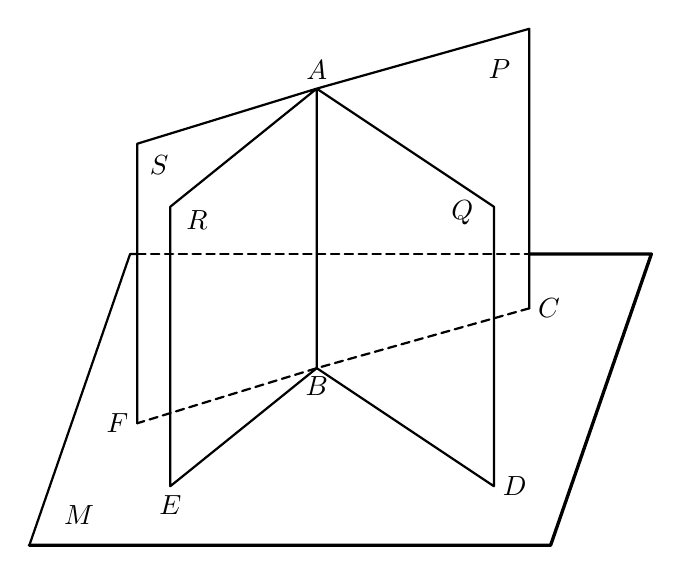
\begin{tikzpicture}[line cap=round,line join=round,every node/.style={inner sep=3pt}]
    \coordinate (A) at (0,3.45);
    \coordinate (B) at (0,-0.1);
    \coordinate (C) at (2.7,0.66);
    \coordinate (D) at (2.25,-1.6);
    \coordinate (E) at (-1.86,-1.6);
    \coordinate (F) at (-2.28,-0.8);

    \draw[thick] (-3.65,-2.35) -- (-2.37,1.35) -- (-2.28,1.35);
    \draw[thick,densely dashed] (-2.28,1.35) -- (2.7,1.35);
    \draw[very thick] (-3.65,-2.35) -- (2.97,-2.35) -- (4.25,1.35) -- (2.7,1.35);

    \draw[thick] (A) -- (2.7,4.21) -- (C)
        (A) -- (2.25,1.95) -- (D) -- (B) -- (E) -- (-1.86,1.95) -- (A)
        (A) -- (-2.28,2.75) -- (F)
        (A) -- (B);
    \draw[thick,densely dashed] (C) -- (B) -- (F);

    \node[above] at (A) {\(A\)};
    \node[below] at (B) {\(B\)};
    \node[right] at (C) {\(C\)};
    \node[right] at (D) {\(D\)};
    \node[below] at (E) {\(E\)};
    \node[left] at (F) {\(F\)};
    \node at (2.32,3.7) {\(P\)};
    \node at (1.85,1.87) {\(Q\)};
    \node at (-1.52,1.78) {\(R\)};
    \node at (-2.0,2.48) {\(S\)};
    \node at (-3.02,-1.96) {\(M\)};
\end{tikzpicture}

    \caption{Перпендикуляры к прямой \(AB\)}\label{fig:kiselev-stereo-306}
\end{figure}

Через любые два из этих перпендикуляров, например \(BC\) и \(BD\), проведём плоскость \(M\). По \hyperref[para:perpendicular-plane-criterion]{теореме §~\ref*{para:perpendicular-plane-criterion}} она перпендикулярна \(AB\). Предположим, что один из остальных перпендикуляров, например \(BE\), проведённый в плоскости \(R\), не лежит в плоскости \(M\). Тогда плоскости \(R\) и \(M\) пересекаются по прямой, отличной от \(BE\). Получается, что в плоскости \(R\) через точку \(B\) проходят два перпендикуляра к \(AB\): \(BE\) и прямая пересечения плоскостей \(M\) и \(R\) (\hyperref[para:perpendicular-plane-criterion]{см.~§~\ref*{para:perpendicular-plane-criterion}}). Это невозможно. Значит, все проведённые перпендикуляры лежат в плоскости \(R\)\footnote{\emph{Прим.~ред.} В начале доказательства плоскость через \(BC\) и \(BD\) обозначена буквой \(M\).}, которая перпендикулярна \(AB\).

\kiselevparagraph{para:unique-plane-normal-to-line} \textbf{Теорема. Через любую точку пространства можно провести ровно одну плоскость, перпендикулярную данной прямой.}

Рассмотрим два случая: точка лежит на данной прямой или вне её.

\begin{figure}[htbp]
    \centering
    \renewcommand{\thefigure}{307}
    \captionsetup{name=Рис.,labelsep=period}
    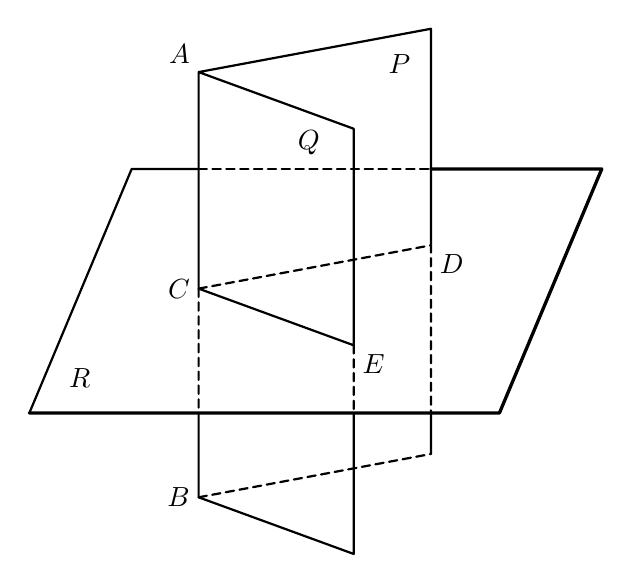
\begin{tikzpicture}[line cap=round,line join=round,every node/.style={inner sep=3pt}]
    \coordinate (A) at (-1.05,2.75);
    \coordinate (B) at (-1.05,-2.65);
    \coordinate (C) at (-1.05,0);
    \coordinate (D) at (1.9,0.55);
    \coordinate (E) at (0.92,-0.72);
    \coordinate (Pbottom) at (1.9,-2.1);
    \coordinate (Qbottom) at (0.92,-3.37);

    \draw[thick] (-1.05,1.52) -- (-1.9,1.52) -- (-3.2,-1.58);
    \draw[thick,densely dashed] (-1.05,1.52) -- (1.9,1.52);
    \draw[very thick] (-3.2,-1.58) -- (2.77,-1.58) -- (4.07,1.52) -- (1.9,1.52);

    \draw[thick] (D) -- (1.9,3.3) -- (A) -- (0.92,2.03) -- (E) -- (C) -- (A);
    \draw[thick,densely dashed] (C) -- (D) -- (1.9,-1.58)
        (C) -- (-1.05,-1.58) (E) -- (0.92,-1.58) (B) -- (Pbottom);
    \draw[thick] (-1.05,-1.58) -- (B) -- (Qbottom) -- (0.92,-1.58)
        (1.9,-1.58) -- (Pbottom);

    \node[above left] at (A) {\(A\)};
    \node[left] at (B) {\(B\)};
    \node[left] at (C) {\(C\)};
    \node[below right] at (D) {\(D\)};
    \node[below right] at (E) {\(E\)};
    \node at (1.5,2.85) {\(P\)};
    \node at (0.35,1.85) {\(Q\)};
    \node at (-2.56,-1.14) {\(R\)};
\end{tikzpicture}

    \caption{Плоскость \(R\), перпендикулярная прямой \(AB\)}\label{fig:kiselev-stereo-307}
\end{figure}

\begin{enumerate}[label=\arabic*),ref=\arabic*]
    \item\label{item:normal-plane-point-on-line} Пусть точка \(C\) лежит на данной прямой \(AB\) (рис.~\ref{fig:kiselev-stereo-307}). Проведём через \(AB\) две плоскости \(P\) и \(Q\), а в них --- прямые \(CD\) и \(CE\), перпендикулярные \(AB\). Через эти пересекающиеся прямые проведём плоскость \(R\).
    % Печатная с. 278.
    Эта плоскость перпендикулярна \(AB\) в точке \(C\), поскольку \(CD\) и \(CE\) перпендикулярны \(AC\)\footnote{\emph{Прим.~ред.} На рис.~\ref{fig:kiselev-stereo-307} точки \(A\), \(B\) и \(C\) лежат на одной прямой.}. Следовательно, любая третья прямая плоскости \(R\), проходящая через \(C\), также перпендикулярна \(AB\) (\hyperref[para:perpendicular-plane-criterion]{см.~§~\ref*{para:perpendicular-plane-criterion}}).

    Чтобы доказать единственность этой плоскости, предположим, что через \(C\) проходит другая плоскость \(R_1\), перпендикулярная \(AB\). Она должна пересекать \(P\) по прямой, проходящей через \(C\) и перпендикулярной \(AB\). В плоскости \(P\) такая прямая только одна --- \(CD\). Значит, обе плоскости \(R_1\) и \(R\) пересекают \(P\) по \(CD\). Так же убедимся, что обе они пересекают плоскость \(Q\) по \(CE\). Следовательно, \(R_1\) и \(R\) проходят через одни и те же пересекающиеся прямые \(CD\) и \(CE\) и потому сливаются в одну (\hyperref[item:plane-through-intersecting-lines]{см.~§~\ref*{para:plane-uniqueness-corollaries}, пункт~\ref*{item:plane-through-intersecting-lines}}).

    \item\label{item:normal-plane-point-outside-line} Пусть точка \(D\) лежит вне данной прямой \(AB\) (рис.~\ref{fig:kiselev-stereo-307}). Проведём через \(D\) и \(AB\) плоскость \(P\), а через \(AB\) --- ещё одну плоскость \(Q\). В плоскости \(P\) опустим из точки \(D\) перпендикуляр \(DC\) на \(AB\), а в плоскости \(Q\) проведём из точки \(C\) перпендикуляр \(CE\) к \(AB\). Плоскость \(R\), проходящая через \(DC\) и \(CE\), проходит через \(D\) и перпендикулярна \(AB\) (\hyperref[para:perpendicular-plane-criterion]{см.~§~\ref*{para:perpendicular-plane-criterion}}).

    Предположим, что через \(D\) проходит ещё одна плоскость \(R_1\), перпендикулярная \(AB\). Она должна пересекать \(P\) по прямой, проходящей через \(D\) и перпендикулярной \(AB\). В плоскости \(P\) такая прямая только одна --- \(DC\).
    % Печатная с. 279.
    Значит, обе плоскости \(R_1\) и \(R\) пересекают \(P\) по \(DC\). В частности, \(R_1\) проходит через \(C\) и потому пересекает \(Q\) по \(CE\), единственной прямой плоскости \(Q\), проходящей через \(C\) и перпендикулярной \(AB\). Таким образом, \(R_1\) и \(R\) проходят через одни и те же пересекающиеся прямые \(DC\) и \(CE\) и сливаются в одну.
\end{enumerate}

\kiselevparagraph{para:unique-line-normal-to-plane} \textbf{Теорема. Через любую точку пространства можно провести ровно один перпендикуляр к данной плоскости.}

Рассмотрим два случая: точка лежит в данной плоскости или вне её.

\begin{enumerate}[label=\arabic*),ref=\arabic*]
    \item\label{item:normal-line-point-in-plane} Пусть точка \(O\) лежит в плоскости \(P\) (рис.~\ref{fig:kiselev-stereo-308}). Проведём через неё в этой плоскости произвольную прямую \(MN\), а затем через \(O\) проведём плоскость \(Q\), перпендикулярную \(MN\) (\hyperref[item:normal-plane-point-on-line]{см.~§~\ref*{para:unique-plane-normal-to-line}, пункт~\ref*{item:normal-plane-point-on-line}}). Пусть \(P\) и \(Q\) пересекаются по прямой \(AB\). В плоскости \(Q\) проведём \(OC\perp AB\). Докажем, что \(OC\) --- перпендикуляр к плоскости \(P\).

    \begin{figure}[htbp]
        \centering
        \renewcommand{\thefigure}{308}
        \captionsetup{name=Рис.,labelsep=period}
        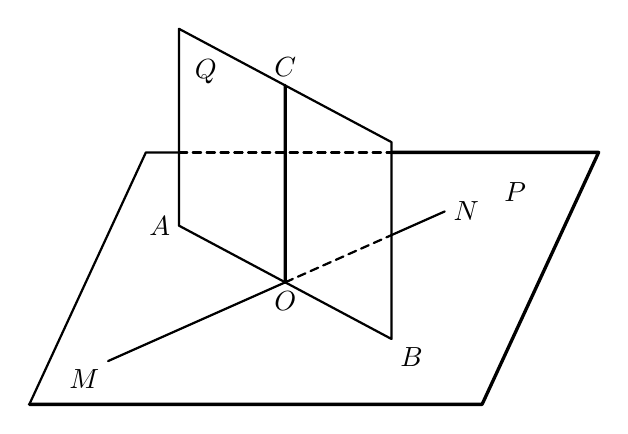
\begin{tikzpicture}[line cap=round,line join=round,every node/.style={inner sep=3pt}]
    \coordinate (A) at (-1.3,0.72);
    \coordinate (B) at (1.4,-0.72);
    \path (A) -- (B) coordinate[midway] (O);
    \coordinate (C) at (0.05,2.5);
    \coordinate (M) at (-2.2,-1);
    \coordinate (N) at (2.075,0.9);
    \coordinate (Qedge) at (1.4,0.6);

    \draw[thick] (-3.2,-1.55) -- (-1.72,1.65) -- (-1.3,1.65);
    \draw[thick,densely dashed] (-1.3,1.65) -- (1.4,1.65);
    \draw[very thick] (-3.2,-1.55) -- (2.55,-1.55) -- (4.03,1.65) -- (1.4,1.65);

    \draw[thick] (A) -- (-1.3,3.22) -- (1.4,1.78) -- (B) -- cycle;
    \draw[very thick] (O) -- (C);
    \draw[thick] (M) -- (O) (Qedge) -- (N);
    \draw[thick,densely dashed] (O) -- (Qedge);

    \node[left] at (A) {\(A\)};
    \node[below right] at (B) {\(B\)};
    \node[above] at (C) {\(C\)};
    \node[below left] at (M) {\(M\)};
    \node[right] at (N) {\(N\)};
    \node[below] at (O) {\(O\)};
    \node at (2.97,1.15) {\(P\)};
    \node at (-0.96,2.67) {\(Q\)};
\end{tikzpicture}

        \caption{Прямая \(OC\) --- перпендикуляр к плоскости \(P\)}\label{fig:kiselev-stereo-308}
    \end{figure}

    Поскольку \(MN\) перпендикулярна плоскости \(Q\), она перпендикулярна любой прямой этой плоскости, проходящей через \(O\). В частности, \(OC\perp MN\). По построению \(OC\perp AB\). Значит, \(OC\) перпендикулярна двум прямым плоскости \(P\), проведённым через \(O\), и потому перпендикулярна самой плоскости (\hyperref[para:perpendicular-plane-criterion]{см.~§~\ref*{para:perpendicular-plane-criterion}}).

    Предположим, что через \(O\) проходит ещё один перпендикуляр \(OC_1\) к плоскости \(P\) (рис.~\ref{fig:kiselev-stereo-309}).
    % Печатная с. 280.
    Проведём через \(OC\) и \(OC_1\) плоскость, которая пересечёт \(P\) по прямой \(OH\). Эта плоскость на рисунке не показана. Тогда углы \(COH\) и \(C_1OH\) должны быть прямыми. Это невозможно, поскольку один из этих углов составляет часть другого. Значит, другого перпендикуляра к \(P\) через точку \(O\) провести нельзя.

    \begin{figure}[htbp]
        \centering
        \renewcommand{\thefigure}{309}
        \captionsetup{name=Рис.,labelsep=period}
        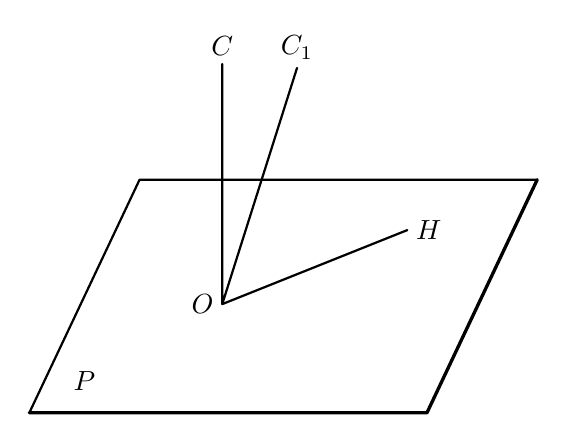
\begin{tikzpicture}[line cap=round,line join=round,every node/.style={inner sep=3pt}]
    \coordinate (O) at (-0.55,0);
    \coordinate (C) at (-0.55,3.05);
    \coordinate (C1) at (0.4,3.0);
    \coordinate (H) at (1.8,0.94);

    \draw[thick] (-3,-1.38) -- (-1.6,1.58) -- (3.45,1.58);
    \draw[very thick] (-3,-1.38) -- (2.05,-1.38) -- (3.45,1.58);
    \draw[thick] (C) -- (O) -- (C1) (O) -- (H);

    \node[left] at (O) {\(O\)};
    \node[above] at (C) {\(C\)};
    \node[above] at (C1) {\(C_1\)};
    \node[right] at (H) {\(H\)};
    \node at (-2.3,-0.98) {\(P\)};
\end{tikzpicture}

        \caption{Предположение о другом перпендикуляре \(OC_1\) через точку \(O\)}\label{fig:kiselev-stereo-309}
    \end{figure}

    \item\label{item:normal-line-point-outside-plane} Пусть точка \(O\) лежит вне плоскости \(P\) (рис.~\ref{fig:kiselev-stereo-310}). Проведём в плоскости \(P\) произвольную прямую \(MN\), а через \(O\) --- плоскость \(Q\), перпендикулярную \(MN\) (\hyperref[item:normal-plane-point-outside-line]{см.~§~\ref*{para:unique-plane-normal-to-line}, пункт~\ref*{item:normal-plane-point-outside-line}}). Пусть \(P\) и \(Q\) пересекаются по прямой \(AB\). В плоскости \(Q\) проведём \(OC\perp AB\). Докажем, что \(OC\) --- перпендикуляр к плоскости \(P\).

    \begin{figure}[htbp]
        \centering
        \renewcommand{\thefigure}{310}
        \captionsetup{name=Рис.,labelsep=period}
        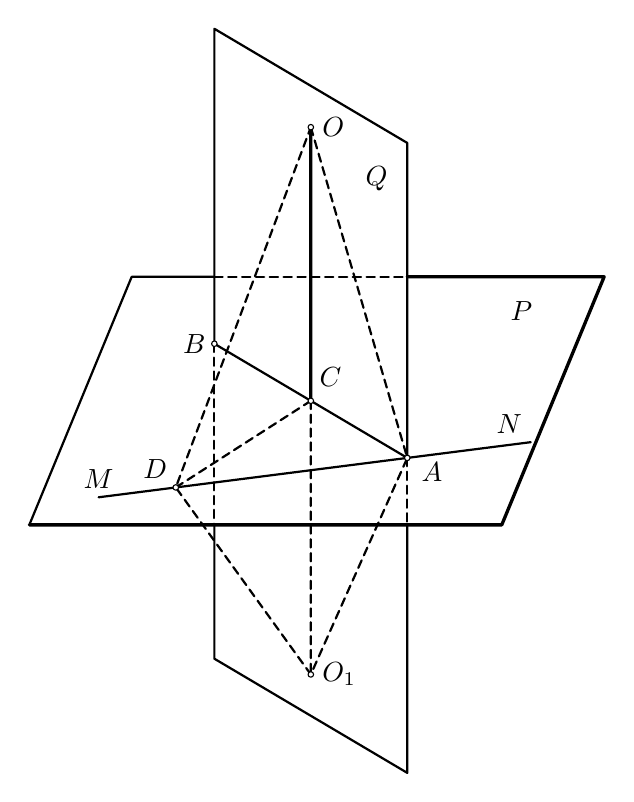
\begin{tikzpicture}[line cap=round,line join=round,every node/.style={inner sep=3pt}]
    \coordinate (A) at (1.55,-0.7);
    \coordinate (B) at (-0.9,0.75);
    \path (A) -- (B) coordinate[midway] (C);
    \coordinate (O) at (0.325,3.5);
    \coordinate (O1) at (0.325,-3.45);
    \coordinate (M) at (-2.37,-1.2);
    \coordinate (N) at (3.118,-0.5);
    \path (M) -- (A) coordinate[pos=0.25] (D);

    \draw[thick] (-3.25,-1.55) -- (-1.95,1.6) -- (-0.9,1.6);
    \draw[thick,densely dashed] (-0.9,1.6) -- (1.55,1.6);
    \draw[very thick] (-3.25,-1.55) -- (2.75,-1.55) -- (4.05,1.6) -- (1.55,1.6);

    \draw[thick] (B) -- (-0.9,4.75) -- (1.55,3.3) -- (A)
        (-0.9,-1.55) -- (-0.9,-3.25) -- (1.55,-4.7) -- (1.55,-1.55);
    \draw[thick,densely dashed] (B) -- (-0.9,-1.55) (A) -- (1.55,-1.55);
    \draw[thick] (B) -- (A) (M) -- (N);
    \draw[thick,densely dashed] (O) -- (A) -- (O1) -- (D) -- (O) (D) -- (C);
    \draw[very thick] (O) -- (C);
    \draw[thick,densely dashed] (C) -- (O1);

    \foreach \point in {A,B,C,D,O,O1} {
        \filldraw[fill=white] (\point) circle[radius=1pt];
    }
    \node[right,xshift=2pt,yshift=-5pt] at (A) {\(A\)};
    \node[left] at (B) {\(B\)};
    \node[above right,yshift=2pt] at (C) {\(C\)};
    \node[above left] at (D) {\(D\)};
    \node[above] at (M) {\(M\)};
    \node[above left] at (N) {\(N\)};
    \node[right,inner sep=4pt] at (O) {\(O\)};
    \node[right,inner sep=4pt] at (O1) {\(O_1\)};
    \node at (3,1.16) {\(P\)};
    \node at (1.16,2.85) {\(Q\)};
\end{tikzpicture}

        \caption{Перпендикуляр \(OC\) из точки \(O\) вне плоскости \(P\)}\label{fig:kiselev-stereo-310}
    \end{figure}

    Достаточно показать, что \(OC\) перпендикулярна двум прямым, проведённым в плоскости \(P\) через \(C\). Одной такой прямой служит \(AB\), которой \(OC\) перпендикулярна по построению. Второй возьмём прямую \(CD\), соединяющую \(C\) с произвольной точкой \(D\) прямой \(MN\).

    Чтобы доказать, что \(OC\perp CD\), продолжим \(OC\) на отрезок \(CO_1=OC\) и соединим точки \(O\) и \(O_1\) с \(A\) и \(D\). Так как \(MN\perp Q\), прямая \(MN\) перпендикулярна \(AO\) и \(AO_1\). Поэтому треугольники \(OAD\) и \(O_1AD\) прямоугольные при вершине \(A\). Катет \(AD\) у них общий. Катеты \(AO\) и \(AO_1\) равны как наклонные, проведённые в плоскости \(Q\) из точки \(A\) к прямой \(OO_1\), поскольку расстояния от их оснований до основания перпендикуляра \(AC\) (отрезки \(OC\) и \(O_1C\)) равны (\kiselevPlanimetryPage{53}{см.~Планиметрия, §~59, пункт~2}). Из равенства этих треугольников следует, что \(OD=O_1D\).

    Треугольники \(OCD\) и \(O_1CD\) равны, поскольку их стороны соответственно равны.
    % Печатная с. 281.
    Значит, \(\angle OCD=\angle O_1CD\), и потому эти углы прямые. Итак, \(OC\perp CA\) и \(OC\perp CD\), следовательно, \(OC\perp P\).

    Предположим, что из \(O\) можно опустить на плоскость \(P\) другой перпендикуляр \(OC_1\) (рис.~\ref{fig:kiselev-stereo-311}). Соединим \(C\) и \(C_1\). Тогда у треугольника \(OCC_1\) два угла, при вершинах \(C\) и \(C_1\), должны быть прямыми. Это невозможно, поэтому второго перпендикуляра из \(O\) к плоскости \(P\) провести нельзя.

    \begin{figure}[htbp]
        \centering
        \renewcommand{\thefigure}{311}
        \captionsetup{name=Рис.,labelsep=period}
        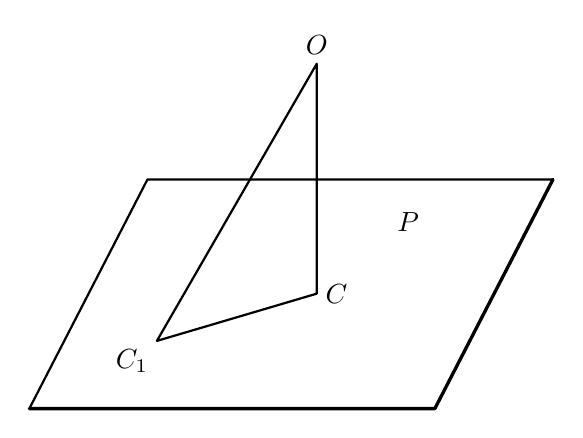
\begin{tikzpicture}[line cap=round,line join=round,every node/.style={inner sep=3pt}]
    \coordinate (O) at (0.5,2.92);
    \coordinate (C) at (0.5,0);
    \coordinate (C1) at (-1.53,-0.6);

    \draw[thick] (-3.15,-1.46) -- (-1.65,1.45) -- (3.5,1.45);
    \draw[very thick] (-3.15,-1.46) -- (2,-1.46) -- (3.5,1.45);
    \draw[thick] (O) -- (C1) -- (C) -- cycle;

    \node[above] at (O) {\(O\)};
    \node[right] at (C) {\(C\)};
    \node[below left] at (C1) {\(C_1\)};
    \node at (1.66,0.91) {\(P\)};
\end{tikzpicture}

        \caption{Предположение о другом перпендикуляре \(OC_1\) из точки \(O\)}\label{fig:kiselev-stereo-311}
    \end{figure}
\end{enumerate}

\kiselevparagraph{para:normal-and-oblique-lengths} \textbf{Сравнительная длина перпендикуляра и наклонных.} Если из одной точки \(A\) (рис.~\ref{fig:kiselev-stereo-312}) к плоскости проведены перпендикуляр \(AB\) и наклонная \(AC\), то \emph{проекцией наклонной на плоскость} называют прямую \(BC\), проведённую между основаниями перпендикуляра и наклонной.

\begin{figure}[htbp]
    \centering
    \renewcommand{\thefigure}{312}
    \captionsetup{name=Рис.,labelsep=period}
    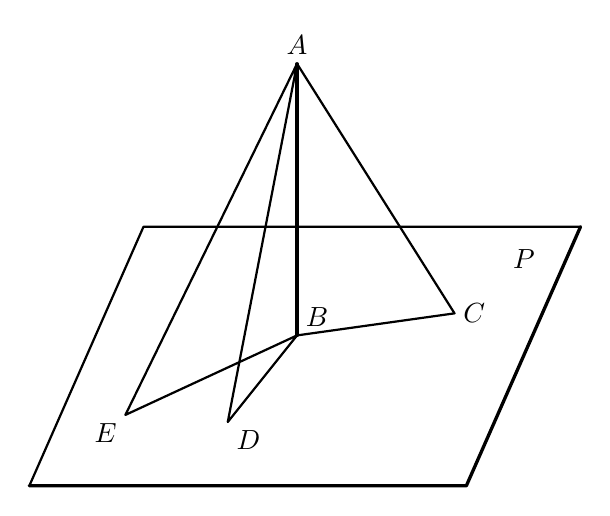
\begin{tikzpicture}[line cap=round,line join=round,every node/.style={inner sep=3pt}]
    \coordinate (A) at (0,3.45);
    \coordinate (B) at (0,0);
    \coordinate (C) at (2,0.28);
    \coordinate (D) at (-0.88,-1.1);
    \coordinate (E) at (-2.18,-1.01);

    \draw[thick] (-3.4,-1.91) -- (-1.95,1.38) -- (3.6,1.38);
    \draw[very thick] (-3.4,-1.91) -- (2.15,-1.91) -- (3.6,1.38);
    \draw[very thick] (A) -- (B);
    \draw[thick] (A) -- (C) -- (B) -- (D) -- (A) -- (E) -- (B);

    \node[above] at (A) {\(A\)};
    \node[above right] at (B) {\(B\)};
    \node[right] at (C) {\(C\)};
    \node[below right] at (D) {\(D\)};
    \node[below left] at (E) {\(E\)};
    \node at (2.88,0.97) {\(P\)};
\end{tikzpicture}

    \caption{Сравнительная длина перпендикуляра и наклонных}\label{fig:kiselev-stereo-312}
\end{figure}

\textbf{Теоремы. Если из одной и той же точки} \(A\)\textbf{, взятой вне плоскости} \(P\) \textbf{(рис.~\ref{fig:kiselev-stereo-312}), к этой плоскости проведены перпендикуляр} \(AB\) \textbf{и какие-нибудь наклонные} (\(AC\), \(AD\), \(AE,\ldots\))\textbf{, то:}

\begin{enumerate}[label=\arabic*),ref=\arabic*]
    \item \textbf{перпендикуляр короче любой наклонной;}
    \item\label{item:equal-projections-equal-obliques} \textbf{наклонные с равными проекциями равны;}
    \item \textbf{из двух наклонных больше та, у которой больше проекция.}
\end{enumerate}

Вращая прямоугольные треугольники \(ABC\) и \(ABD\) вокруг катета \(AB\), можно совместить их плоскости с плоскостью треугольника \(ABE\). Тогда все наклонные окажутся в одной плоскости с перпендикуляром, а все проекции будут лежать на одной прямой.
% Печатная с. 282.
Таким образом, эти теоремы сводятся к аналогичным теоремам планиметрии (см.~Планиметрия, §~59, \kiselevPlanimetryPage{52}{пункт~1} и \kiselevPlanimetryPage{53}{пункт~2}).

\textbf{Замечание.} \emph{Расстоянием} от точки \(A\) до плоскости \(P\) называют длину перпендикуляра, опущенного из этой точки на плоскость (рис.~\ref{fig:kiselev-stereo-312}).

\kiselevparagraph{para:obliques-determine-projections} \textbf{Обратные теоремы. Если из одной и той же точки вне плоскости провести к этой плоскости перпендикуляр и наклонные, то у равных наклонных проекции равны. Из двух проекций больше та, которая соответствует большей наклонной.}

Доказательство от противного оставляем читателю.

\kiselevparagraph{para:three-perpendiculars} Приведём ещё одну теорему о перпендикулярах, которая понадобится дальше.\footnote{В некоторых курсах геометрии эту теорему или её вариант называют \emph{теоремой трёх перпендикуляров}. Она связывает три перпендикуляра: \(AB\) к плоскости \(P\), \(BC\) к прямой \(DE\) и \(AC\) к той же прямой \(DE\).}

\textbf{Теорема. Прямая} \(DE\) (рис.~\ref{fig:kiselev-stereo-313})\textbf{, проведённая в плоскости} \(P\) \textbf{через основание наклонной} \(AC\) \textbf{перпендикулярно её проекции} \(BC\)\textbf{, перпендикулярна и самой наклонной.}

\begin{figure}[htbp]
    \centering
    \renewcommand{\thefigure}{313}
    \captionsetup{name=Рис.,labelsep=period}
    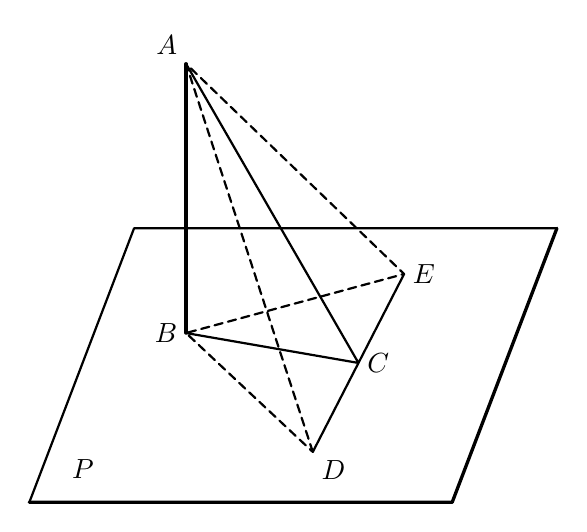
\begin{tikzpicture}[line cap=round,line join=round,every node/.style={inner sep=3pt}]
    \coordinate (A) at (-1.26,3.62);
    \coordinate (B) at (-1.26,0.2);
    \coordinate (D) at (0.35,-1.31);
    \coordinate (E) at (1.51,0.95);
    \path (D) -- (E) coordinate[midway] (C);

    \draw[thick] (-3.25,-1.95) -- (-1.92,1.53) -- (3.45,1.53);
    \draw[very thick] (-3.25,-1.95) -- (2.12,-1.95) -- (3.45,1.53);
    \draw[very thick] (A) -- (B);
    \draw[thick] (A) -- (C) -- (B) (D) -- (E);
    \draw[thick,densely dashed] (D) -- (A) -- (E) -- (B) -- cycle;

    \node[above left] at (A) {\(A\)};
    \node[left] at (B) {\(B\)};
    \node[right] at (C) {\(C\)};
    \node[below right] at (D) {\(D\)};
    \node[right] at (E) {\(E\)};
    \node at (-2.57,-1.53) {\(P\)};
\end{tikzpicture}

    \caption{Теорема трёх перпендикуляров}\label{fig:kiselev-stereo-313}
\end{figure}

Отложим произвольные, но равные отрезки \(CD\) и \(CE\) и соединим точки \(A\) и \(B\) с \(D\) и \(E\). Тогда \(BD=BE\) как наклонные к прямой \(DE\), основания которых одинаково удалены от основания перпендикуляра \(BC\) (\kiselevPlanimetryPage{53}{см.~Планиметрия, §~59, пункт~2}). Значит, \(AD=AE\), поскольку у этих наклонных к плоскости \(P\) равные проекции \(BD\) и \(BE\) (\hyperref[item:equal-projections-equal-obliques]{см.~§~\ref*{para:normal-and-oblique-lengths}, пункт~\ref*{item:equal-projections-equal-obliques}}). Поэтому треугольник \(ADE\) равнобедренный, и его медиана \(AC\) перпендикулярна основанию \(DE\) (\kiselevPlanimetryPage{39}{см.~Планиметрия, §~39}).

\clearpage
\endgroup
